\documentclass{article}

\usepackage{fancyhdr}
\usepackage{extramarks}
\usepackage{amsmath}
\usepackage{amsthm}
\usepackage{amsfonts}
\usepackage{amssymb}
\usepackage{xparse}
\usepackage{tikz}
\usepackage{graphicx}
\usepackage[plain]{algorithm}
\usepackage{algpseudocode}
\usepackage{listings}
\usepackage{hyperref}
\usepackage[per-mode = fraction]{siunitx}
\usepackage{calc}

\usetikzlibrary{automata,positioning}

\hypersetup{
    colorlinks=true,
    linkcolor=blue,
    filecolor=magenta,
    urlcolor=blue,
    }

\urlstyle{same}

%
% Basic Document Settings
%

\topmargin=-0.45in
\evensidemargin=0in
\oddsidemargin=0in
\textwidth=6.5in
\textheight=9.0in
\headsep=0.25in

\linespread{1.1}

\pagestyle{fancy}
\lhead{\hmwkAuthorName}
\chead{\hmwkClass\ (\hmwkClassInstructor,\ \hmwkClassTime): \hmwkTitle}
\rhead{\firstxmark}
\lfoot{\lastxmark}
\cfoot{\thepage}

\renewcommand\headrulewidth{0.4pt}
\renewcommand\footrulewidth{0.4pt}

\setlength\parindent{0pt}
\allowdisplaybreaks
%
% Title Page
%

\title{
	\vspace{2in}
	\textmd{\textbf{\hmwkClass:\ \hmwkTitle}}\\
	\normalsize\vspace{0.1in}\small{Due\ on\ \hmwkDueDate\ at \hmwkDueTime}\\
	\vspace{0.1in}\large{\textit{\hmwkClassInstructor,\ \hmwkClassTime}}
	\vspace{3in}
}
\author{\textbf{\hmwkAuthorName}}
\date{\hmwkCompletionDate}

%
% Create Problem Sections
%

\newcommand{\enterProblemHeader}[1]{
	\nobreak\extramarks{}{Problem #1 continued on next page\ldots}\nobreak{}
	\nobreak\extramarks{Problem #1 (continued)}{Problem #1 continued on next page\ldots}\nobreak{}
}

\newcommand{\exitProblemHeader}[1]{
	\nobreak\extramarks{Problem #1 (continued)}{Problem #1 continued on next page\ldots}\nobreak{}
	\nobreak\extramarks{Problem #1}{}\nobreak{}
}

%
% Homework Problem Environment
%
\NewDocumentEnvironment{hwkProblem}{m m s}{
	\section*{Problem #1: #2}
	\enterProblemHeader{#1}
	\setcounter{partCounter}{1}
}{
	\exitProblemHeader{#1}
	\IfBooleanF{#3} % if star, no new page
		{\newpage}
}

% Alias for the Solution section header
\newcommand{\hwkSol}{\vspace{\baselineskip / 2}\textbf{\Large Solution}\vspace{\baselineskip / 2}}

% Alias for the Solution Part subsection header
\newcounter{partCounter}
\newcommand{\hwkPart}{
	\vspace{\baselineskip / 2}
	\textbf{\large Part \Alph{partCounter}}
	\vspace{\baselineskip / 2}
	\stepcounter{partCounter}
}

%
% Various Helper Commands
%

% Such That
\newcommand{\st}{\text{s.t.}}

% Useful for algorithms
\newcommand{\alg}[1]{\textsc{\bfseries \footnotesize #1}}

% For derivatives
\newcommand{\deriv}[1]{\frac{\mathrm{d}}{\mathrm{d}x} (#1)}

% For partial derivatives
\newcommand{\pderiv}[2]{\frac{\partial}{\partial #1} (#2)}

% Integral dx
\newcommand{\dx}{\mathrm{d}x}
\newcommand{\dy}{\mathrm{d}y}

% Probability commands: Expectation, Variance, Covariance, Bias
\newcommand{\e}[1]{\mathrm{e}#1}
\newcommand{\E}{\mathrm{E}}
\newcommand{\Var}{\mathrm{Var}}
\newcommand{\Cov}{\mathrm{Cov}}
\newcommand{\Bias}{\mathrm{Bias}}

% Defining Units that are not in the SI base
\DeclareSIUnit\bar{bar}
\DeclareSIUnit\ft{ft}
\DeclareSIUnit\dollar{\$}
\DeclareSIUnit\cent{\text{\textcent}}
\DeclareSIUnit\c{\degreeCelsius}

% Code Listing config
\usepackage{xcolor}
\definecolor{codegreen}{rgb}{0,0.6,0}
\definecolor{codegray}{rgb}{0.5,0.5,0.5}
\definecolor{codepurple}{rgb}{0.58,0,0.82}
\definecolor{backcolour}{rgb}{0.95,0.95,0.92}
\lstdefinestyle{overleaf}{
	% backgroundcolor=\color{backcolour},
	commentstyle=\color{codegreen},
	keywordstyle=\color{magenta},
	numberstyle=\tiny\color{codegray},
	stringstyle=\color{codepurple},
	basicstyle=\ttfamily\footnotesize,
	breakatwhitespace=false,
	breaklines=true,
	captionpos=b,
	keepspaces=true,
	numbers=left,
	numbersep=5pt,
	showspaces=false,
	showstringspaces=false,
	showtabs=false,
	tabsize=4
}

\usepackage[latte]{catppuccinpalette}
\lstdefinestyle{catppuccin}{
	breaklines=true,
	keepspaces=true,
	numbers=left,
	numbersep=5pt,
	showspaces=false,
	showstringspaces=false,
	breakatwhitespace=true,
	tabsize=4,
	stringstyle = {\color{CtpGreen}},
	commentstyle={\color{CtpOverlay1}},
	basicstyle = {\small\color{CtpText}\ttfamily},
	keywordstyle = {\color{CtpMauve}},
	keywordstyle = [2]{\color{CtpBlue}},
	keywordstyle = [3]{\color{CtpYellow}},
	keywordstyle = [4]{\color{CtpLavender}},
	keywordstyle = [5]{\color{CtpPeach}},
	keywordstyle = [6]{\color{CtpTeal}}
}

\lstset{style=catppuccin}


%
% Homework Details
%   - Title
%   - Due date
%   - Due time
%   - Course
%   - Section/Time
%   - Instructor
%   - Author
%

\newcommand{\hmwkTitle}{Homework 04}
\newcommand{\hmwkSubTitle}{}
\newcommand{\hmwkDueDate}{March 10th, 2025}
\newcommand{\hmwkDueTime}{03:30 PM}
\newcommand{\hmwkClass}{ENRE 447 - 0101}
\newcommand{\hmwkClassTime}{03:30 PM}
\newcommand{\hmwkClassInstructor}{Dr. Groth}
\newcommand{\hmwkAuthorName}{\textbf{Vai Srivastava}}
\newcommand{\hmwkCompletionDate}{\today}

\begin{document}

\maketitle

\pagebreak

\begin{hwkProblem}{1}{}

	Nine light bulbs are observed, and the exact failure time of each is recorded as 70, 150, 250, 360, 485, 650, 855, 1130, and 1540. Estimate and plot the following:
	\begin{enumerate}
		\item Cdf of failure times
		\item Pdf of failure times
		\item Reliability function
		\item Hazard-rate function
	\end{enumerate}

	\hwkSol

	\begin{align*}
		\hat{F}(t) &= \frac{1}{9}\sum_{i=1}^{9} \mathbf{1}\{t_i\le t\},\\[1mm]
		\hat{f}(t) &\approx \text{KDE estimate of } f(t),\\[1mm]
		\hat{R}(t) &= 1-\hat{F}(t),\\[1mm]
		\hat{h}(t) &= \frac{\hat{f}(t)}{\hat{R}(t)}. \quad \qed
	\end{align*}

	\begin{figure}[H]
		\begin{center}
			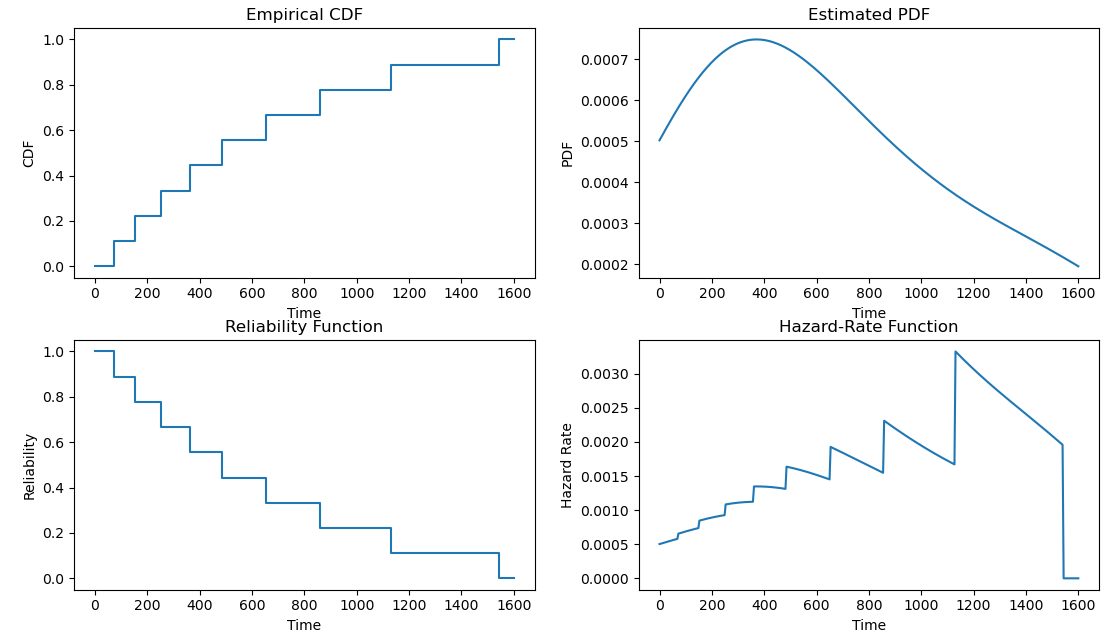
\includegraphics[width=0.8\textwidth]{./images/s01.png}
		\end{center}
		\caption{Plot for HW04 P01}\label{fig:s01}
	\end{figure}
	
	
	\hwkCode

	\lstinputlisting[language=python, caption={Python code for HW04 P01}, label={lst:s01}]{./code/s01.py}

\end{hwkProblem}

\begin{hwkProblem}{2}{}

	The following time to failure data are found when 158 transformer units are put under test. No failures are observed prior to 1750 hours.
	\begin{center}
		\begin{tabular}{lcccccc}
			Time Interval: & \( 1750 \to 2250 \) & \( 2250 \to 2750 \) & \( 2750 \to 3250 \) & \( 3250 \to 3750 \) & \( 3750 \to 4250 \) & \( 4250 \to 4750 \) \\
			\# Failures: & 17 & 54 & 27 & 17 & 19 & 24
		\end{tabular}
	\end{center}
	Use a nonparametric method to estimate \( \func{f}[t], \func{h}[t], \) and \( \func{R}[t] \) of the transformers.

	\hwkSol

	Define:
	\begin{align*}
		n_1 &= 158,\quad n_2 = 158 - 17 = 141,\quad n_3 = 141 - 54 = 87,\\[1mm]
		n_4 &= 87 - 27 = 60,\quad n_5 = 60 - 17 = 43,\quad n_6 = 43 - 19 = 24,\\[1mm]
		\Delta t &= 500 \text{ (hours)}.
	\end{align*}
	The piecewise constant density is estimated by
	\begin{align*}
		\hat{f}(t) &= \begin{cases}
			\frac{17}{158\cdot500}, & 1750\le t<2250,\\[1mm]
			\frac{54}{141\cdot500}, & 2250\le t<2750,\\[1mm]
			\frac{27}{87\cdot500},  & 2750\le t<3250,\\[1mm]
			\frac{17}{60\cdot500},  & 3250\le t<3750,\\[1mm]
			\frac{19}{43\cdot500},  & 3750\le t<4250,\\[1mm]
			\frac{24}{24\cdot500},  & 4250\le t<4750,
		\end{cases}\\[1mm]
		\hat{R}(t) &= \begin{cases}
			1, & 1750\le t<2250,\\[1mm]
			\frac{141}{158}, & 2250\le t<2750,\\[1mm]
			\frac{87}{158}, & 2750\le t<3250,\\[1mm]
			\frac{60}{158}, & 3250\le t<3750,\\[1mm]
			\frac{43}{158}, & 3750\le t<4250,\\[1mm]
			\frac{24}{158}, & 4250\le t<4750,\\[1mm]
			0, & t\ge4750,
		\end{cases}\\[1mm]
		\hat{h}(t) &= \frac{\hat{f}(t)}{\hat{R}(t)}. \quad \qed
	\end{align*}

\end{hwkProblem}

\begin{hwkProblem}{3}{}

	Time to failure data from eight devices placed on an accelerated test is shown below.
	\begin{center}
		\begin{tabular}{lcccccccc}
			i: & 1 & 2 & 3 & 4 & 5 & 6 & 7 & 8 \\
			TTF: & 65 & 85 & 90 & 95 & 340 & 405 & 555 & 575
		\end{tabular}
	\end{center}
	\begin{enumerate}
		\item Use probability plotting to estimate the parameter of the exponential distribution.
		\item Discuss the suitability of the explonential distribution for this data.
	\end{enumerate}

	\hwkSol

	\begin{align*}
		\bar{t} &= \frac{65+85+90+95+340+405+555+575}{8} = 276.25,\\[1mm]
		\hat{\lambda} &= \frac{1}{\bar{t}} \approx \frac{1}{276.25} \approx 0.00362,\\[1mm]
		\text{Exponential CDF:}\quad F(t) &= 1 - e^{-\lambda t},\\[1mm]
		\ln(-\ln(1-F(t))) &= \ln(\lambda) + \ln t.
	\end{align*}
	A probability plot of $\ln(-\ln(1-\hat{F}(t)))$ versus $\ln t$ should be linear with slope 1.

	\begin{align*}
		\text{Thus, } \hat{\lambda} &\approx 0.00362.\\[1mm]
		\text{(Discussion: Deviations from linearity indicate that the exponential model} &\text{ may not be fully suitable.)} \quad \qed
	\end{align*}

	\begin{figure}[H]
		\begin{center}
			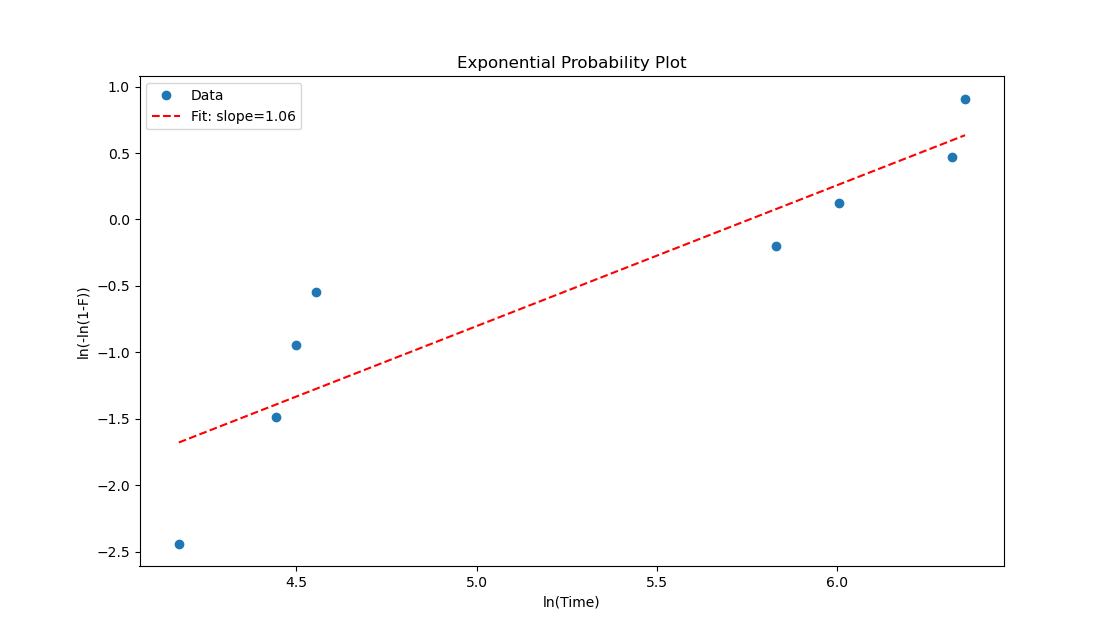
\includegraphics[width=0.8\textwidth]{./images/s03.png}
		\end{center}
		\caption{Plot for HW04 P03}\label{fig:s03}
	\end{figure}

	\hwkCode

	\lstinputlisting[language=python, caption={Python code for HW04 P03}, label={lst:s03}]{./code/s03.py}

\end{hwkProblem}

\begin{hwkProblem}{4}{}

	In an accelerated test, failures of 8 units are recorded after 8, 17, 21, 21, 22, 39, 42, and 47 days after starting in operation. The other two units are operating after 50 days.
	\begin{enumerate}
		\item Perform a Weibull probability plot of these data.
		\item Find the parameters of the Weibull distribution from the plot.
	\end{enumerate}

	\hwkSol

	Using only the 8 failures, assign median rank estimates:
	\begin{align*}
		\hat{F}(t_{(i)}) &\approx \frac{i-0.3}{8+0.4},\quad i=1,\ldots,8,\\[1mm]
		\ln\bigl[-\ln(1-\hat{F}(t_{(i)}))\bigr] &= \beta\,\ln(t_{(i)}) - \beta\,\ln(\eta).
	\end{align*}
	A linear regression of
	\[
		Y_i=\ln\bigl[-\ln(1-\hat{F}(t_{(i)}))\bigr] \quad \text{versus} \quad X_i=\ln(t_{(i)})
	\]
	yields slope $\hat{\beta}$ and intercept $-\hat{\beta}\ln(\eta)$. From the plot one obtains, approximately,
	\begin{align*}
		\hat{\beta} &\approx 1.82 \quad \qed \\
		\hat{\eta} &\approx 31.5 \quad \qed
	\end{align*}

	\begin{figure}[H]
		\begin{center}
			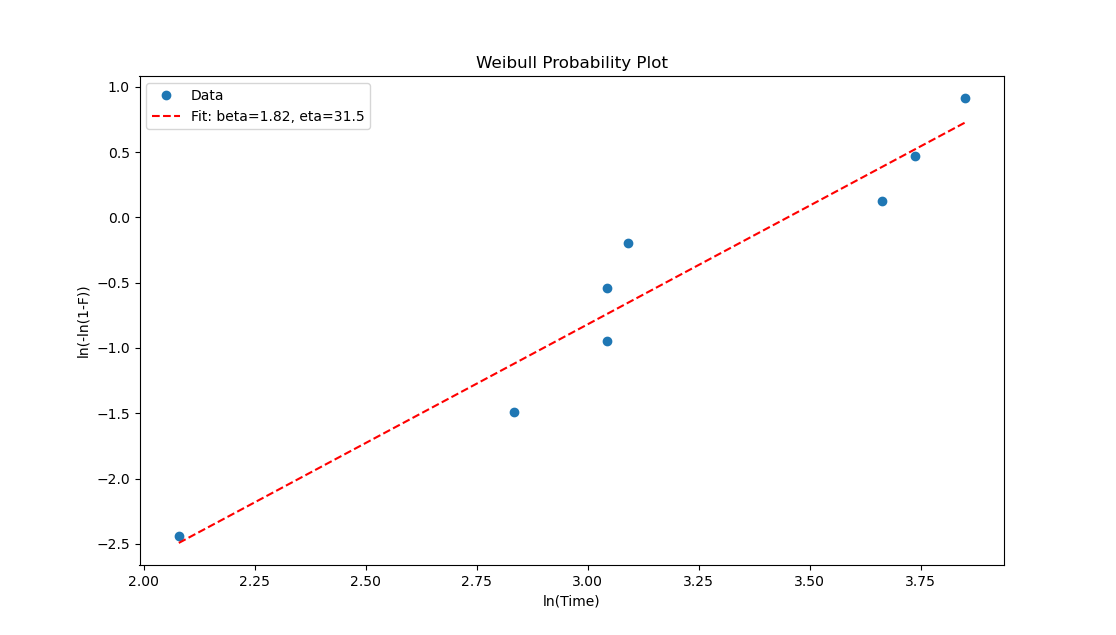
\includegraphics[width=0.8\textwidth]{./images/s04.png}
		\end{center}
		\caption{Plot for HW04 P04}\label{fig:s04}
	\end{figure}

	\hwkCode

	\lstinputlisting[language=python, caption={Python code for HW04 P04}, label={lst:s04}]{./code/s04.py}

\end{hwkProblem}

\end{document}
